\section{Results of the Runtime Verified AV System}

This research provides a solution for two aspects of \acf{AV} systems: predicting accurately with perturbations to the system's inputs and safely dealing with misclassifications by the system.
The issue of input perturbations was addressed using a \acf{SNN} of different convolutional \acfp{SANN}, each \ac{SANN} working in tandem to predict more accurately.
Misclassification by the system's controller was addressed by implementing sensor fusion between cameras and \ac{LiDAR}.
This was done using a run-time enforcer that enforced a safety automaton.

To test the \ac{SNN}'s ability to deal with perturbations, the input images (taken from the \ac{VOC} 2012 and \ac{GTSRB} datasets) were perturbed by randomly replacing approximately 7\% of the image pixels with randomly coloured pixels.
Figure~\ref{fig:sign-graph-acc} shows that the input perturbations decreased the accuracy of the classifiers by as much as 50\%, a huge amount.
However, the aim of this approach is not only to increase the classification accuracy of the \acp{SNN} but rather catch misclassifications made by the \acp{SANN}, i.e. verify that the classifications made by the \acp{SANN} are valid.
As such the results displayed don't show an increase in accuracy, but rather that the enforcer is fully capable of catching misclassifications made by the \acp{SNN}.
Table~\ref{tbl:sign-resultsfull} shows that without input perturbations, the enforcer caught about 70\% of all misclassifications. 
This is a huge amount, more than half of all the misclassifications made were detected by the enforcer, and the safety of the system turned over to the driver.
This same table show that when the inputs are perturbed, the enforcer picks up more misclassifications than with the original images, averaging at around 80\% of all misclassifications.
Where input perturbations are concerned, the enforcer responds even better and picks up the majority of the total misclassifications.
Figure~\ref{fig:sign-graphboth} presents these results in a graphical format, showing that the enforcer performs even better under more unpredictable circumstances.

\begin{table}[ht]
	\centering
	\resizebox{\textwidth}{!}{%
		\begin{tabular}{|p{0.2\linewidth}||p{0.2\linewidth}|p{0.2\linewidth}|p{0.2\linewidth}|}
			\hline
			Epochs trained & No. of misclassifications (/100) & No. of caught misclassifications (/100) & \% of total misclassifications caught \\ \hline
			\multicolumn{4}{|l|}{Original Inputs} \\ \hline
			0 & 95.16 & 95.16 & 100 \\ 
			10 & 95.16 & 95.16 & 100 \\
			100 & 82.67 & 61.09 & 73.90 \\
			1000 & 29.36 & 21.39 & 72.85 \\
			10000 & 12.38 & 8.55 & 69.06 \\ 
			100000 & 11.98 & 7.79 & 65.03 \\
			6000 (best) & 10.59 & 7.32 & 69.12 \\ \hline
			\multicolumn{4}{|l|}{Perturbed Inputs} \\ \hline
			0 & 95.16 & 95.16 & 100 \\
			10 & 95.16 & 95.16 & 100 \\ 
			100 & 93.63 & 71.89 & 76.78 \\
			1000 & 76.69 & 63.71 & 83.07 \\
			10000 & 57.89 & 45.89 & 79.27 \\ 
			100000 & 58.03 & 45.72 & 78.79 \\
			7000 (best) & 60.42 & 49.13 & 81.31 \\ \hline
		\end{tabular}%
	}
	\caption{Table showing the results of the \ac{AV} prediction \ac{SNN}}
	\label{tbl:sign-resultsfull}
\end{table}

\begin{figure}[t]
	\centering
	\scalebox{0.9}{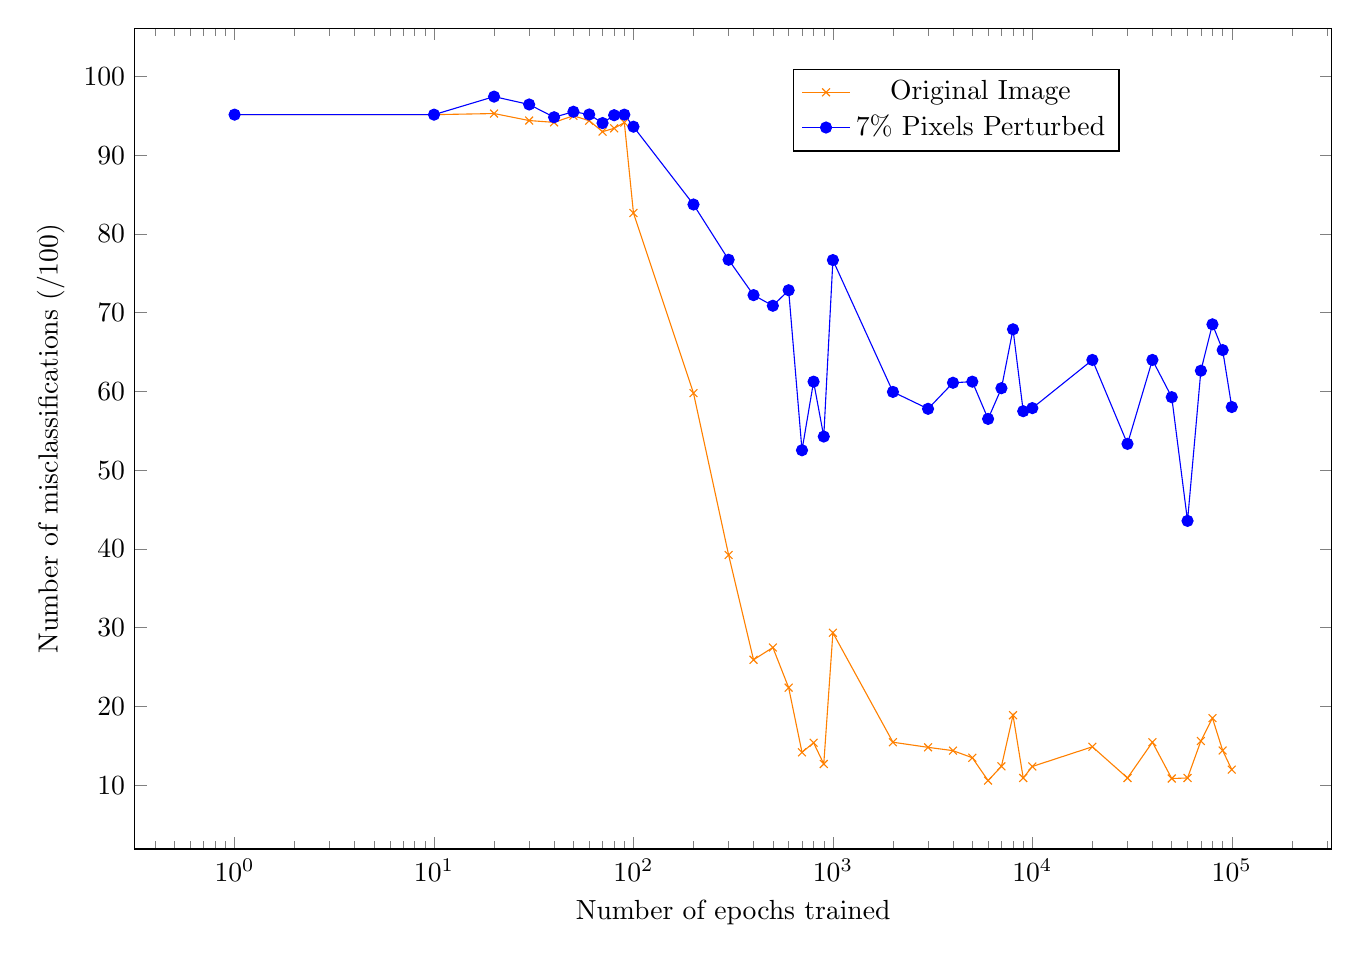
\begin{tikzpicture}
\begin{semilogxaxis}[
xlabel={Number of epochs trained},
ylabel={Number of misclassifications (/100)},
x=1.1cm,
y=1.0mm, 
legend style={at={(0.55,0.9)},anchor=west}]

\addplot[color=orange,mark=x] coordinates {
	(1, 95.159996)
	(10, 95.159996)
	(20, 95.300003)
	(30, 94.410004)
	(40, 94.180000)
	(50, 95.019997)
	(60, 94.389999)
	(70, 93.000000)
	(80, 93.419998)
	(90, 94.159996)
	(100, 82.669998)
	(200, 59.790001)
	(300, 39.240002)
	(400, 25.930000)
	(500, 27.490000)
	(600, 22.389999)
	(700, 14.180000)
	(800, 15.390000)
	(900, 12.700000)
	(1000, 29.359999)
	(2000, 15.460000)
	(3000, 14.810000)
	(4000, 14.390000)
	(5000, 13.490000)
	(6000, 10.590000)
	(7000, 12.400000)
	(8000, 18.889999)
	(9000, 10.920000)
	(10000, 12.380000)
	(20000, 14.880000)
	(30000, 10.920000)
	(40000, 15.460000)
	(50000, 10.850000)
	(60000, 10.920000)
	(70000, 15.620001)
	(80000, 18.520000)
	(90000, 14.410000)
	(100000, 11.980000)
};

\addplot[color=blue,mark=*] coordinates {
	(1, 95.159996)
	(10, 95.159996)
	(20, 97.450005)
	(30, 96.450005)
	(40, 94.830002)
	(50, 95.529999)
	(60, 95.180000)
	(70, 94.089996)
	(80, 95.089996)
	(90, 95.159996)
	(100, 93.629997)
	(200, 83.750000)
	(300, 76.729996)
	(400, 72.239998)
	(500, 70.889999)
	(600, 72.860001)
	(700, 52.540001)
	(800, 61.250000)
	(900, 54.280003)
	(1000, 76.689995)
	(2000, 59.950001)
	(3000, 57.799999)
	(4000, 61.109997)
	(5000, 61.250000)
	(6000, 56.520000)
	(7000, 60.420002)
	(8000, 67.900002)
	(9000, 57.500000)
	(10000, 57.889999)
	(20000, 64.010002)
	(30000, 53.349998)
	(40000, 64.010002)
	(50000, 59.280003)
	(60000, 43.570000)
	(70000, 62.639999)
	(80000, 68.529999)
	(90000, 65.259995)
	(100000, 58.029999)
};


\legend{Original Image, 7\% Pixels Perturbed}
\end{semilogxaxis}%
\end{tikzpicture}%}
	\caption{Line graph showing the effect of input perturbations on the prediction accuracy of a \ac{SNN} \label{fig:sign-graph-acc}}
\end{figure}

%\begin{figure}[t]
%	\centering
%	\scalebox{0.9}{\begin{tikzpicture}
\begin{semilogxaxis}[
xlabel={Number of epochs trained},
ylabel={\% of total classifications},
x=1.1cm,
y=1.0mm, 
legend style={at={(0.55,0.9)},anchor=west}]

\addplot[color=black,mark=x] coordinates {
	(1, 100.000000)
	(10, 100.000000)
	(20, 99.968513)
	(30, 99.438622)
	(40, 98.948822)
	(50, 99.831619)
	(60, 100.000000)
	(70, 99.946243)
	(80, 98.629845)
	(90, 99.235352)
	(100, 73.896217)
	(200, 67.904327)
	(300, 73.114166)
	(400, 71.500191)
	(500, 73.917786)
	(600, 72.264412)
	(700, 71.438644)
	(800, 70.175438)
	(900, 70.787399)
	(1000, 72.854225)
	(2000, 70.439842)
	(3000, 69.480080)
	(4000, 67.477409)
	(5000, 68.717560)
	(6000, 69.121811)
	(7000, 70.645164)
	(8000, 67.972473)
	(9000, 68.772896)
	(10000, 69.063011)
	(20000, 67.405907)
	(30000, 69.780220)
	(40000, 67.787842)
	(50000, 69.032257)
	(60000, 68.315018)
	(70000, 68.693977)
	(80000, 70.194382)
	(90000, 69.604439)
	(100000, 65.025040)
};

\addplot[color=brown,mark=x] coordinates {	
	(1, 0.000000)
	(10, 0.000000)
	(20, 0.031486)
	(30, 0.561380)
	(40, 1.051184)
	(50, 0.168381)
	(60, 0.000000)
	(70, 0.053759)
	(80, 1.370155)
	(90, 0.764649)
	(100, 26.103786)
	(200, 32.095673)
	(300, 26.885832)
	(400, 28.499805)
	(500, 26.082212)
	(600, 27.735594)
	(700, 28.561354)
	(800, 29.824560)
	(900, 29.212601)
	(1000, 27.145777)
	(2000, 29.560154)
	(3000, 30.519920)
	(4000, 32.522587)
	(5000, 31.282434)
	(6000, 30.878185)
	(7000, 29.354836)
	(8000, 32.027523)
	(9000, 31.227106)
	(10000, 30.936995)
	(20000, 32.594090)
	(30000, 30.219782)
	(40000, 32.212166)
	(50000, 30.967743)
	(60000, 31.684982)
	(70000, 31.306025)
	(80000, 29.805618)
	(90000, 30.395559)
	(100000, 34.974957)
};


\legend{Caught misclassifications, Uncaught misclassifications}
\end{semilogxaxis}%
\end{tikzpicture}%}
%	\caption{Line graph showing the performance of the system trained over an increasing amount of epochs using unperturbed inputs \label{fig:sign-graph}}
%\end{figure}

%\begin{figure}[t]
%	\centering
%	\scalebox{0.9}{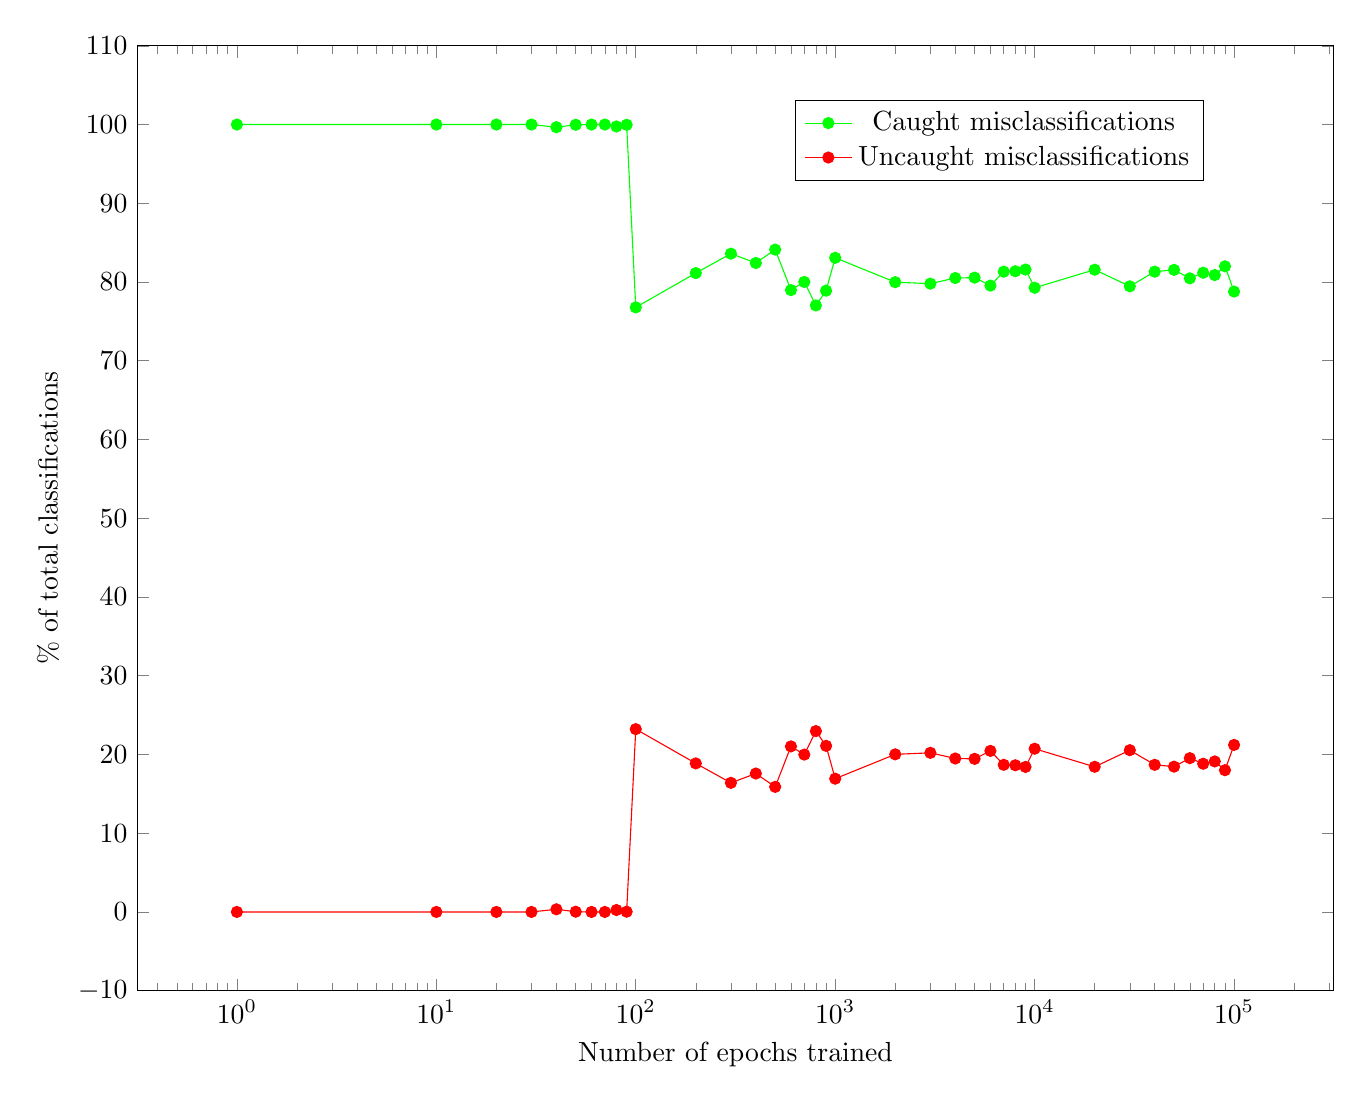
\begin{tikzpicture}
\begin{semilogxaxis}[
xlabel={Number of epochs trained},
ylabel={\% of total classifications},
x=1.1cm,
y=1.0mm, 
legend style={at={(0.55,0.9)},anchor=west}]

\addplot[color=green,mark=*] coordinates {	
	(1, 100.000000)
	(10, 100.000000)
	(20, 100.000000)
	(30, 100.000000)
	(40, 99.662552)
	(50, 99.968597)
	(60, 100.000000)
	(70, 100.000000)
	(80, 99.758133)
	(90, 99.968475)
	(100, 76.780945)
	(200, 81.134331)
	(300, 83.604851)
	(400, 82.419716)
	(500, 84.116234)
	(600, 78.973373)
	(700, 80.015221)
	(800, 77.028572)
	(900, 78.905663)
	(1000, 83.074722)
	(2000, 79.983315)
	(3000, 79.792389)
	(4000, 80.510559)
	(5000, 80.555107)
	(6000, 79.547066)
	(7000, 81.314125)
	(8000, 81.369659)
	(9000, 81.582603)
	(10000, 79.271027)
	(20000, 81.565376)
	(30000, 79.456421)
	(40000, 81.315414)
	(50000, 81.545204)
	(60000, 80.468216)
	(70000, 81.178162)
	(80000, 80.884285)
	(90000, 81.995102)
	(100000, 78.786835)
};

\addplot[color=red,mark=*] coordinates {
	(1, 0.000000)
	(10, 0.000000)
	(20, 0.000000)
	(30, 0.000000)
	(40, 0.337446)
	(50, 0.031402)
	(60, 0.000000)
	(70, 0.000000)
	(80, 0.241872)
	(90, 0.031525)
	(100, 23.219051)
	(200, 18.865665)
	(300, 16.395145)
	(400, 17.580284)
	(500, 15.883766)
	(600, 21.026627)
	(700, 19.984774)
	(800, 22.971428)
	(900, 21.094332)
	(1000, 16.925280)
	(2000, 20.016680)
	(3000, 20.207613)
	(4000, 19.489441)
	(5000, 19.444899)
	(6000, 20.452932)
	(7000, 18.685873)
	(8000, 18.630341)
	(9000, 18.417391)
	(10000, 20.728970)
	(20000, 18.434624)
	(30000, 20.543579)
	(40000, 18.684584)
	(50000, 18.454794)
	(60000, 19.531784)
	(70000, 18.821840)
	(80000, 19.115713)
	(90000, 18.004898)
	(100000, 21.213161)
};

\legend{Caught misclassifications, Uncaught misclassifications}
\end{semilogxaxis}%
\end{tikzpicture}%}
%	\caption{Line graph showing the number of misclassifications made by the system with perturbed inputs \label{fig:sign-graphpert}}
%\end{figure}

\begin{figure}[t]
	\centering
	\scalebox{0.9}{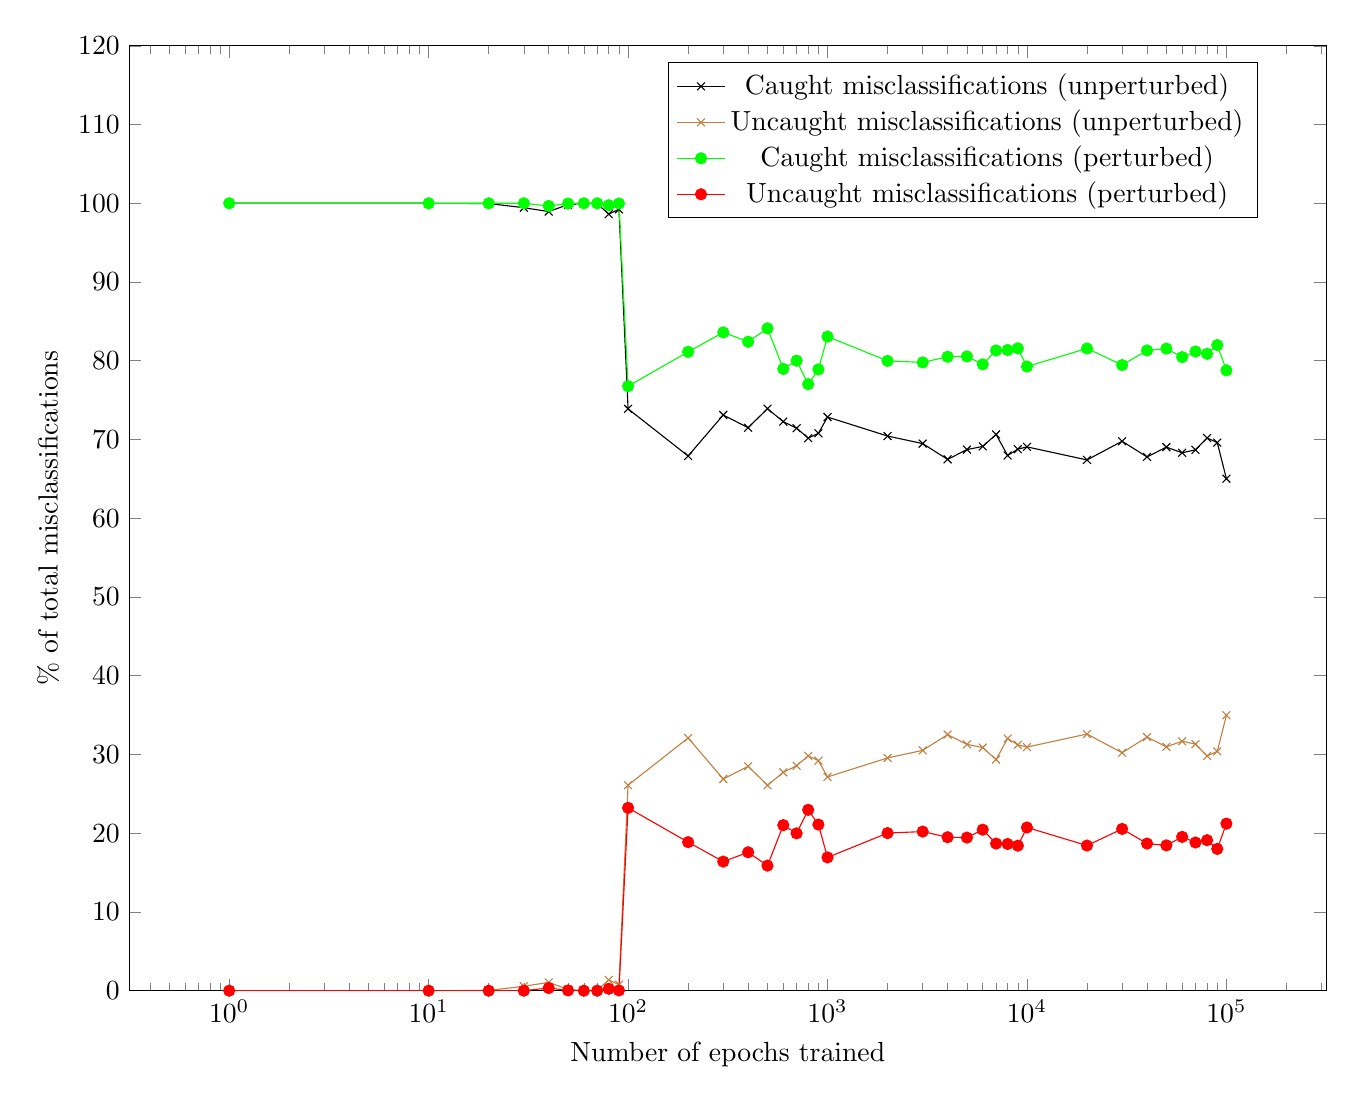
\begin{tikzpicture}
\begin{semilogxaxis}[
xlabel={Number of epochs trained},
ylabel={\% of total misclassifications},
x=1.1cm, y=1.0mm, 
ymin=0, ymax=120,
legend style={at={(0.45,0.9)},anchor=west}]

\addplot[color=black,mark=x] coordinates {
	(1, 100.000000)
	(10, 100.000000)
	(20, 99.968513)
	(30, 99.438622)
	(40, 98.948822)
	(50, 99.831619)
	(60, 100.000000)
	(70, 99.946243)
	(80, 98.629845)
	(90, 99.235352)
	(100, 73.896217)
	(200, 67.904327)
	(300, 73.114166)
	(400, 71.500191)
	(500, 73.917786)
	(600, 72.264412)
	(700, 71.438644)
	(800, 70.175438)
	(900, 70.787399)
	(1000, 72.854225)
	(2000, 70.439842)
	(3000, 69.480080)
	(4000, 67.477409)
	(5000, 68.717560)
	(6000, 69.121811)
	(7000, 70.645164)
	(8000, 67.972473)
	(9000, 68.772896)
	(10000, 69.063011)
	(20000, 67.405907)
	(30000, 69.780220)
	(40000, 67.787842)
	(50000, 69.032257)
	(60000, 68.315018)
	(70000, 68.693977)
	(80000, 70.194382)
	(90000, 69.604439)
	(100000, 65.025040)
};

\addplot[color=brown,mark=x] coordinates {	
	(1, 0.000000)
	(10, 0.000000)
	(20, 0.031486)
	(30, 0.561380)
	(40, 1.051184)
	(50, 0.168381)
	(60, 0.000000)
	(70, 0.053759)
	(80, 1.370155)
	(90, 0.764649)
	(100, 26.103786)
	(200, 32.095673)
	(300, 26.885832)
	(400, 28.499805)
	(500, 26.082212)
	(600, 27.735594)
	(700, 28.561354)
	(800, 29.824560)
	(900, 29.212601)
	(1000, 27.145777)
	(2000, 29.560154)
	(3000, 30.519920)
	(4000, 32.522587)
	(5000, 31.282434)
	(6000, 30.878185)
	(7000, 29.354836)
	(8000, 32.027523)
	(9000, 31.227106)
	(10000, 30.936995)
	(20000, 32.594090)
	(30000, 30.219782)
	(40000, 32.212166)
	(50000, 30.967743)
	(60000, 31.684982)
	(70000, 31.306025)
	(80000, 29.805618)
	(90000, 30.395559)
	(100000, 34.974957)
};

\addplot[color=green,mark=*] coordinates {	
	(1, 100.000000)
	(10, 100.000000)
	(20, 100.000000)
	(30, 100.000000)
	(40, 99.662552)
	(50, 99.968597)
	(60, 100.000000)
	(70, 100.000000)
	(80, 99.758133)
	(90, 99.968475)
	(100, 76.780945)
	(200, 81.134331)
	(300, 83.604851)
	(400, 82.419716)
	(500, 84.116234)
	(600, 78.973373)
	(700, 80.015221)
	(800, 77.028572)
	(900, 78.905663)
	(1000, 83.074722)
	(2000, 79.983315)
	(3000, 79.792389)
	(4000, 80.510559)
	(5000, 80.555107)
	(6000, 79.547066)
	(7000, 81.314125)
	(8000, 81.369659)
	(9000, 81.582603)
	(10000, 79.271027)
	(20000, 81.565376)
	(30000, 79.456421)
	(40000, 81.315414)
	(50000, 81.545204)
	(60000, 80.468216)
	(70000, 81.178162)
	(80000, 80.884285)
	(90000, 81.995102)
	(100000, 78.786835)
};

\addplot[color=red,mark=*] coordinates {
	(1, 0.000000)
	(10, 0.000000)
	(20, 0.000000)
	(30, 0.000000)
	(40, 0.337446)
	(50, 0.031402)
	(60, 0.000000)
	(70, 0.000000)
	(80, 0.241872)
	(90, 0.031525)
	(100, 23.219051)
	(200, 18.865665)
	(300, 16.395145)
	(400, 17.580284)
	(500, 15.883766)
	(600, 21.026627)
	(700, 19.984774)
	(800, 22.971428)
	(900, 21.094332)
	(1000, 16.925280)
	(2000, 20.016680)
	(3000, 20.207613)
	(4000, 19.489441)
	(5000, 19.444899)
	(6000, 20.452932)
	(7000, 18.685873)
	(8000, 18.630341)
	(9000, 18.417391)
	(10000, 20.728970)
	(20000, 18.434624)
	(30000, 20.543579)
	(40000, 18.684584)
	(50000, 18.454794)
	(60000, 19.531784)
	(70000, 18.821840)
	(80000, 19.115713)
	(90000, 18.004898)
	(100000, 21.213161)
};

\legend{Caught misclassifications (unperturbed), Uncaught misclassifications (unperturbed), Caught misclassifications (perturbed), Uncaught misclassifications (perturbed)}
\end{semilogxaxis}%
\end{tikzpicture}%}
	\caption{Line graph showing the number of misclassifications caught by the enforcer \label{fig:sign-graphboth}}
\end{figure}

%\todo{Add table showing how \ac{SNN} affects the prediction accuracy}

\subsection{An \ac{AV} System Using \acf{MNN2C}}
\ac{MNN2C}, introduced in Section~\ref{sec:mnn2c}, creates time-predictable, modular \acfp{SNN} for C from existing Keras (with Tensorflow) trained \acp{ANN}. 
This compiler makes implementing \acfp{SNN} in C easy and safe.
For the purposes of testing and demonstration, the complex \ac{SNN} used in this chapter, shown in Figure~\ref{fig:mnn}, was trained in Python, using Keras and the exact same images used to train the original system.
This \ac{SNN} was then described in the \ac{MNN2C} format, and modular C code was generated to initialise, run and incorporate the \ac{SNN}.
To show the efficacy of \ac{MNN2C}, the generated \ac{SNN} was implemented in an identical system to the original, and run with the same tests. 
It has already been shown that \ac{MNN2C} generates outputs identical to the Keras trained \acp{ANN} with a one hundred-thousandth tolerance, so the output of each individual \ac{ANN} is not being tested, rather that the system as a whole runs as the original does.

\subsubsection{Results of an \ac{MNN2C} Generated \ac{AV} System}
Figure~\ref{fig:sign-graphboth-mnn2c} shows that the enforcer stills runs perfectly fine with Keras trained \acp{SNN} compiled to C code.
The enforcer picked up more than 70\% of all misclassifications, catching more misclassifications as the training of the \acp{SNN} was increased. 
As the training increased, the \acp{SNN} become more confident with their predictions, and thus the enforcer is able to more accurately determine misclassifications.

Since these \acp{SNN} were trained in Keras, they did not need to go through extensive training to get to a reasonable classification accuracy, only needing 100 epochs to get to level as the Darknet \acp{SNN}.
The enforcer works very similarly for perturbed and unperturbed images, unlike the Darknet \acp{SNN}.
This is due to the effective training methods used by Keras, allowing for better trained \acp{SNN} even with input perturbations.

%\begin{figure}[t]
%	\centering
%	\scalebox{0.9}{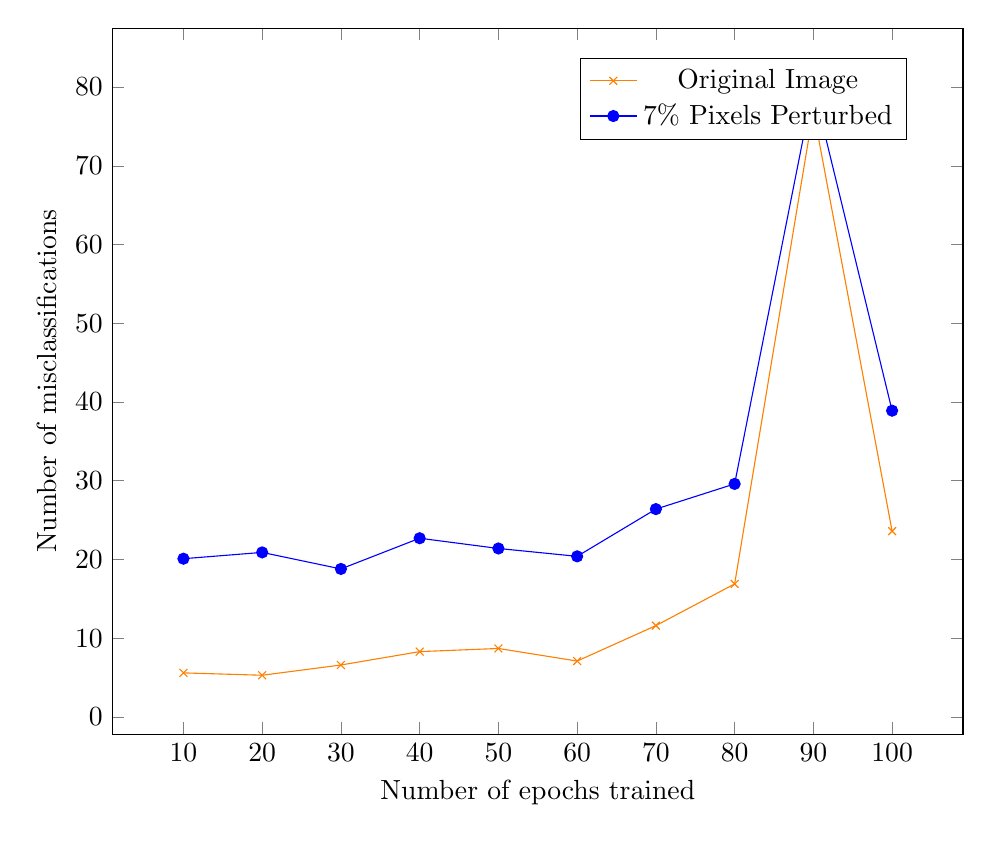
\begin{tikzpicture}
\begin{axis}[
xlabel={Number of epochs trained},
ylabel={Number of misclassifications},
x=1.0mm,
y=1.0mm, 
legend style={at={(0.55,0.9)},anchor=west}]

\addplot[color=orange,mark=x] coordinates {
	(10, 5.600000)
	(20, 5.300000)
	(30, 6.600000)
	(40, 8.300000)
	(50, 8.700000)
	(60, 7.100000)
	(70, 11.600000)
	(80, 16.900000)
	(90, 77.000000)
	(100, 23.600000)
	
};

\addplot[color=blue,mark=*] coordinates {
	(10, 20.100000)
	(20, 20.900000)
	(30, 18.799999)
	(40, 22.700001)
	(50, 21.400000)
	(60, 20.400000)
	(70, 26.400000)
	(80, 29.600000)
	(90, 80.000000)
	(100, 38.900002)
};


\legend{Original Image, 7\% Pixels Perturbed}
\end{axis}%
\end{tikzpicture}%}
%	\caption{Line graph showing the effect of input perturbations on the prediction accuracy of a \ac{SNN} \label{fig:sign-graph-acc-mnn2c}}
%\end{figure}

\begin{figure}[t]
	\centering
	\scalebox{0.9}{\begin{tikzpicture}
\begin{axis}[
xlabel={Number of epochs trained},
ylabel={\% of total misclassifications},
x=1.5mm, y=1.0mm, 
ymin=0, ymax=120,
legend style={at={(0.45,0.9)},anchor=west}]

\addplot[color=black,mark=x] coordinates {
	(10, 71.428574)
	(20, 75.471695)
	(30, 68.181816)
	(40, 84.337349)
	(50, 85.057472)
	(60, 73.239433)
	(70, 84.482758)
	(80, 98.816566)
	(90, 98.181816)
	(100, 97.033897)
};

\addplot[color=green,mark=*] coordinates {	
	(10, 78.109451)
	(20, 65.550240)
	(30, 62.765957)
	(40, 76.651985)
	(50, 82.710281)
	(60, 77.450981)
	(70, 83.712120)
	(80, 95.945946)
	(90, 95.750000)
	(100, 95.372749)
};

\legend{Caught misclassifications (unperturbed), Caught misclassifications (perturbed)}
\end{axis}%
\end{tikzpicture}%}
	\caption{Line graph showing the number of misclassifications caught by the enforcer with \ac{MNN2C} generated \acp{SNN} \label{fig:sign-graphboth-mnn2c}}
\end{figure}





















